\documentclass[12pt]{article}

%***************************************************************************************************
% Math
\usepackage{fancyhdr} 
\usepackage{amsfonts}
\usepackage{amsmath}
\usepackage{amssymb}
\usepackage{amsthm}
%\usepackage{dsfont}

%***************************************************************************************************
% Macros
\usepackage{calc}

%***************************************************************************************************
% Commands and Custom Variables	
\newcommand{\problem}[1]{\hspace{-4 ex} \large \textbf{Problem #1} }
\let\oldemptyset\emptyset
\let\emptyset\varnothing
\newcommand{\norm}[1]{\left\lVert#1\right\rVert}
\newcommand{\sint}{\text{s}\kern-5pt\int}
\newcommand{\powerset}{\mathcal{P}}
\renewenvironment{proof}{\hspace{-4 ex} \emph{Proof}:}{\qed}
\newcommand{\RR}{\mathbb{R}}
\newcommand{\NN}{\mathbb{N}}
\newcommand{\QQ}{\mathbb{Q}}
\newcommand{\ZZ}{\mathbb{Z}}
\newcommand{\CC}{\mathbb{C}}


%***************************************************************************************************
%page
\usepackage[margin=1in]{geometry}
\usepackage{setspace}
%\doublespacing
\allowdisplaybreaks
\pagestyle{fancy}
\fancyhf{}
\rhead{Shaw \space \thepage}
\setlength\parindent{0pt}

%***************************************************************************************************
%Code
\usepackage{listings}
\usepackage{courier}
\lstset{
	language=Python,
	showstringspaces=false,
	formfeed=newpage,
	tabsize=4,
	commentstyle=\itshape,
	basicstyle=\ttfamily,
}

%***************************************************************************************************
%Images
\usepackage{graphicx}
\graphicspath{ {images/} }
\usepackage{float}

%tikz
\usepackage[utf8]{inputenc}
\usepackage{pgfplots}
\usepgfplotslibrary{groupplots}

%***************************************************************************************************
%Hyperlinks
%\usepackage{hyperref}
%\hypersetup{
%	colorlinks=true,
%	linkcolor=blue,
%	filecolor=magenta,      
%	urlcolor=cyan,
%}

\begin{document}
	\thispagestyle{empty}
	
	\begin{flushright}
		Sage Shaw \\
		m565 - Fall 2017 \\
		\today
	\end{flushright}
	
{\large \textbf{HW 5}}\bigbreak

\problem{1 (Natural cubic spline) (a)} 

	From our natural end condition we know that $s_1^{\prime\prime}(x_2)=0$. Thus \\$-\tfrac{3}{2} + 6d_1(4-3) = 0$ gives us that $d_1 = \tfrac{1}{4}$. Since $s_1$ interpolates the point $(4,0)$ we know that $s_1(4)=0$ so 

	\begin{align*}
		0 & = 1 + b_1(4-3) - \tfrac{3}{4}(4-3)^2 + \tfrac{1}{4}(4-3)^3\\
		& = \tfrac{1}{2} + b_1 \\
		-\tfrac{1}{2} & = b_1
	\end{align*}

	Frome the condition that $s_0^{\prime\prime}(3) = s_1^{\prime\prime}(3)$ we have that
	\begin{align*}
		s_0^{\prime\prime}(3) & = s_1^{\prime\prime}(3) \\
		6d_0(3-1) & = -\tfrac{3}{2} + 6d_1(3-3) \\
		d_0 & = -\tfrac{1}{8}
	\end{align*}

	From the condition that $s_0^\prime(3) = s_1^\prime(3)$ we have
	\begin{align*}
		s_0^\prime(3) & = s_1^\prime(3)\\
		b_0 - \tfrac{3}{8}(3-1)^2 & = b_1 = -\tfrac{1}{2} \\
		b_0 & = 1
	\end{align*}
	
	Thus our values are $b_0 = 1, d_0 =-\tfrac{1}{8}, b_1 = -\tfrac{1}{2}$, and $ d_1 = \tfrac{1}{4}$. 
	
\problem{1 (b)} Using the Newton's divided difference table we have

	\begin{center}
		\begin{tabular}{|c|c|c|c|}\hline
			$x_i$ & $f[\cdot]$ & $f[\cdot,\cdot]$ & $f[\cdot,\cdot,\cdot]$ \\ \hline
			1 & 0 & & \\ \hline
			3 & 1 & $\tfrac{1}{2}$ &\\ \hline
			4 & 0 & -1 & $0-\tfrac{1}{2}$ \\ \hline
		\end{tabular}
	\end{center}
	so our global interpolating polynomial is 
	$$
	p_2 = 0 + \tfrac{1}{2}(x-1) - \tfrac{1}{2}(x-1)(x-3) = \tfrac{1}{2}(-4+5x-x^2)
	$$
	Then
	\begin{align*}
		\int_1^4 [s^{\prime\prime}(x)]^2 dx & = \int_1^3 [s_0^{\prime\prime}(x)]^2 dx + \int_3^4 [s_1^{\prime\prime}(x)]^2 dx \\
		& = \int_1^3 [-\tfrac{6}{8}(x-1)]^2 dx + \int_3^4 [-\tfrac{3}{2} + \tfrac{3}{2}(x-3)]^2 dx \\
		& = \int_1^3 \tfrac{9}{16}(x-1)^2 dx + \int_3^4 [\tfrac{3}{2}(x-4)]^2 dx \\
		& = \int_1^3 \tfrac{9}{16}(x-1)^2 dx + \int_3^4 \tfrac{9}{4}(x-4)^2 dx \\
		& = \tfrac{3}{16}(x-1)^3 \Big\vert_1^3 + \tfrac{3}{4}(x-4)^3 \Big\vert_3^4 \\
		& = \tfrac{3}{2} + \tfrac{3}{4} \\
		& = \tfrac{9}{4}
	\end{align*}
	and 
	\begin{align*}
		\int_1^4 [p_2^{\prime\prime}(x)]^2 dx & = \int_1^4 [\tfrac{1}{2}(-2)]^2 dx \\
		& = \int_1^4 1 dx \\
		& = 3
	\end{align*}
	Indeed $\int_1^4 [s^{\prime\prime}(x)]^2 dx < \int_1^4 [p_2^{\prime\prime}(x)]^2 dx$.
	
\problem{2 (Periodic Cubic Spline) (a)}
	
	As in the general case for $k = 1, ..., n-1$ we have
	$$
	h_kd_{k-1} + 2(h_{k+1} + h_{k})d_k + h_{k-1}d_{k+1} = 3(h_k\delta_{k-1} + h_{k-1}\delta_{k})
	$$
	In order to solve the system we need two more equations which we will get from our periodic end conditions. From the condition $s_0^\prime(x_0) = s_{n-1}^\prime(x_n)$ we know that $d_0 = d_n$. From $s_0^{\prime\prime}(x_0) = s_{n-1}^{\prime\prime}(x_n)$ we know that
	\begin{align*}
		2c_0 & = 2c_{n-1} + 6b_{n-1}h_{n-1} \\
		c_0h_0h_{n-1} & = c_{n-1}h_0h_{n-1} + 3b_{n-1}h_{n-1}h_0h_{n-1} \\
		(3\delta_0 - 2d_0 - d_1)h_{n-1} & = (3\delta_{n-1} - 2d_{n-1} - d_n)h_{0} + 3(d_{n-1} -2\delta_{n-1} + d_n)h_{0} \\
		3(h_{n-1}\delta_0 + h_0\delta_{n-1}) & = 2h_{n-1} d_0 + h_{n-1}d_1 + h_0d_{n-1} + 2h_0d_n 
	\end{align*}
	
\problem{2 (b)}

	From part (a) we have the linear system $A\vec{d} = \vec{b}$
	$$
	\begin{bmatrix}
	1 & & & \dots & -1\\
	h_1 & 2(h_1+h_0) & h_0\\
	& \ddots & \ddots & \ddots \\
	& & h_{n-1} & 2(h_{n-1}+h_{n-2}) & h_{n-2} \\
	2h_{n-1} & h_{n-1} & & h_0 & 2h_0 \\
	\end{bmatrix}
	\begin{bmatrix}
	d_0 \\
	d_1 \\
	d_2 \\
	\vdots \\
	d_{n-1} \\
	d_n \\
	\end{bmatrix}
	=
	\begin{bmatrix}
	0 \\
	3(h_1\delta_{0} + h_{0}\delta_{1}) \\
	3(h_2\delta_{1} + h_{1}\delta_{2}) \\
	\vdots \\
	3(h_{n-1}\delta_{n-2} + h_{n-2}\delta_{n-1}) \\
	3(h_{n-1}\delta_0 + h_0\delta_{n-1}) \\
	\end{bmatrix}	
	$$
	
\problem{2 (c)} Code for periodic piecewise cubic spline:
	\begin{lstlisting}
def piecewise_interp(xs, ys, us):
	#periodic piecewise interpolation
	
	#sort the data
	xs = np.array(xs)
	p = xs.argsort()
	xs = xs[p]
	ys = np.array(ys)[p]
	us = np.sort(us)
	
	n = len(xs)
	hs = xs[1:] - xs[:-1]
	
	delta = (ys[1:] - ys[:-1]) / hs
	
	A = np.zeros( (n,n) )
	for i in range(1, n-1):
		A[i, i-1] = hs[i]
		A[i, i] = 2*(hs[i]+hs[i-1])
		A[i, i+1] = hs[i-1]
	A[n-1, 0] = 2*hs[n-2]
	A[n-1, 1] = hs[n-2]
	A[n-1, n-2] = hs[0]
	A[n-1, n-1] = 2*hs[0]
	
	B = np.zeros( (n, 1) )
	for i in range(1, n-1):
		B[i] = 3*( hs[i]*delta[i-1] + hs[i-1]*delta[i] )
	
	A[0,0] = 1
	A[0,n-1] = -1
	B[n-1] = 3*( hs[-1]*delta[0] + hs[0]*delta[-1] )
	
	d = np.linalg.solve(A, B)
	d.shape = (n,)
	
	b = (d[:-1] -2*delta + d[1:])/(hs*hs)
	c = (3*delta - 2*d[:-1] - d[1:])/(hs)
	
	f = np.zeros( len(us) )
	j = 0
	for i, u in enumerate(us):
		while xs[j+1] < u:
			j += 1
			if j >= n-1:
				j = n-2
				break
		dis = u - xs[j] 
		f[i] = ys[j] + d[j]*dis + c[j]*dis**2 + b[j]*dis**3
	return f
	\end{lstlisting}
	
\problem{2 (d)} In figure (\ref{hw5_p2_fig1}) can be seen sample points of $f(x) = \sin(\pi(x-0.01))$ in blue, the periodic cubic spline in red, and the not-a-knot cubic spline in green. The periodic cubic spline appears to be roughly as good an approximation of $f$ as the not-a-knot cubic spline.

	\begin{figure}[H]
		\caption{Plot of sample points from $f(x)$, the periodic cubic spline, and the not-a-knot cubic spline}
		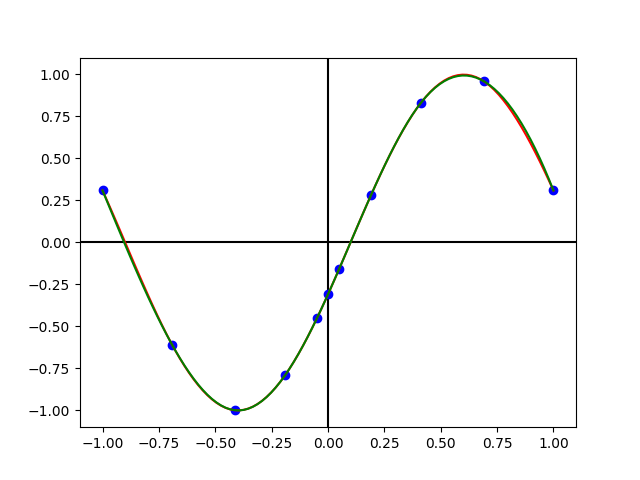
\includegraphics[width=0.80\textwidth]{hw5_p2_fig1}
		\label{hw5_p2_fig1}
		\centering
	\end{figure}


	The code that was used to generate figure (\ref{hw5_p2_fig1}) appears below
	\begin{lstlisting}
def p2d():
	xs = []
	for i in range(0,6):
		xs.append( np.sin(np.pi * i / 10) - 1 )
	for i in range(6, 11):
		xs.append( 1 - np.sin(np.pi * i / 10) )
	xs = np.array(xs)
	ys = np.sin( np.pi*(xs - 0.1) )
	us = np.linspace(-1, 1, 100)
	fs = piecewise_interp(xs, ys, us)
	
	plt.plot( (-100, 100), (0,0), 'k-')
	plt.plot( (0,0), (-100, 100), 'k-')
	plt.plot( xs, ys, 'bo')
	plt.plot( us, fs, 'r-')
	
	cs = CubicSpline(xs,ys)
	plt.plot(us, cs(us), 'g-')
	
	plt.xlim( (-1.1, 1.1) )
	plt.ylim( (-1.1, 1.1) )
	plt.show()
	\end{lstlisting}
	
\problem{3} In figure (\ref{hw5_p3_fig1}) the sample points can be seen in blue, the piecewise-linear interpolation can be seen in green and the periodic cubic spline interpolation can be seen in red.
	
	\begin{figure}[H]
		\caption{Plot of sample points from $f(x)$, the periodic cubic spline, and the not-a-knot cubic spline}
		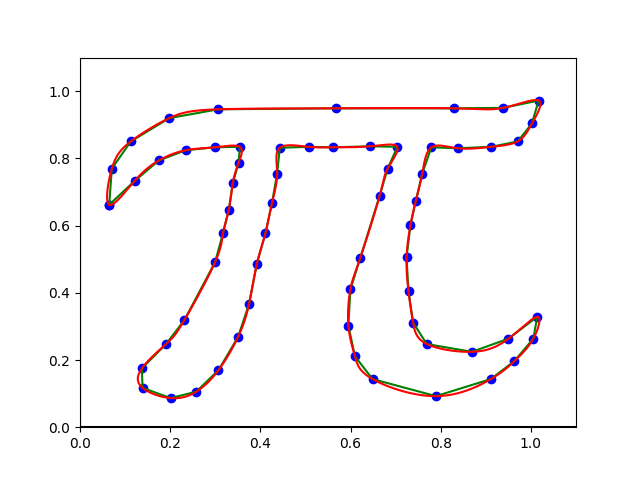
\includegraphics[width=0.80\textwidth]{hw5_p3_fig1}
		\label{hw5_p3_fig1}
		\centering
	\end{figure}
	
	The code that generated figure (\ref{hw5_p3_fig1}) appears below.
	
	\begin{lstlisting}
def p3():
	str = open('res/hw5_DotToDot.txt', 'r').read()
	x = []
	y = []
	for l in str.split('\n'):
		xy = l.split('\t')
		x.append( float(xy[0]))
		y.append( float(xy[1]))
	t = np.linspace(0, 1, len(x))
	u = np.linspace(0, 1, len(x)*100)
	fx = piecewise_interp(t, x, u)
	fy = piecewise_interp(t, y, u)
	
	plt.plot( (-100, 100), (0,0), 'k-')
	plt.plot( (0,0), (-100, 100), 'k-')
	plt.plot( x, y, 'bo')
	plt.plot( x, y, 'g-')
	plt.plot( fx, fy, 'r-')
	
	plt.xlim( (0, 1.1) )
	plt.ylim( (0, 1.1) )
	plt.show()
	\end{lstlisting}
	
	

\end{document}
